\documentclass[paper=letter,fontsize=11pt]{scrartcl} % KOMA-article class
							
\usepackage[english]{babel}
\usepackage[utf8x]{inputenc}
\usepackage[protrusion=true,expansion=true]{microtype}
\usepackage{amsmath,amsfonts,amsthm}     % Math packages
\usepackage{graphicx}                    % Enable pdflatex
\usepackage[svgnames]{xcolor}            % Colors by their 'svgnames'
\usepackage{geometry}

\usepackage{marvosym} % For cool symbols.



	%\textheight=700px                    % Saving trees ;-)
%\usepackage{url}
\usepackage[colorlinks=true,
linkcolor=blue,
urlcolor=blue]{hyperref}
\usepackage{float}
\usepackage{enumerate}
\usepackage{wrapfig}
\usepackage{color}
\usepackage{attachfile}

\frenchspacing              % Better looking spacings after periods
\pagestyle{empty}           % No pagenumbers/headers/footers

%\addtolength{\voffset}{-40pt}
%\addtolength{\textheight}{20pt}

\setlength\topmargin{0pt}
\addtolength\topmargin{-\headheight}
\addtolength\topmargin{-\headsep}
\setlength\oddsidemargin{0pt}
\setlength\textwidth{\paperwidth}
\addtolength\textwidth{-2in}
\setlength\textheight{\paperheight}
%\addtolength\textheight{-3in}
\addtolength\textheight{-2in}
\usepackage{layout}

%%% Custom sectioning}{sectsty package)
%%% ------------------------------------------------------------
\usepackage{sectsty}

\sectionfont{%			            % Change font of \section command
	\usefont{OT1}{phv}{b}{n}%		% bch-b-n: CharterBT-Bold font
	\sectionrule{0pt}{0pt}{-4pt}{2pt}}

%%% Macros
%%% ------------------------------------------------------------
\newlength{\spacebox}
\settowidth{\spacebox}{8888888888}			% Box to align text
\newcommand{\sepspace}{\vspace*{1em}}		% Vertical space macro

\newcommand{\MyName}[1]{ % Name
		\Huge \usefont{OT1}{Imr}{b}{n} \hfill #1
		\par \normalsize \normalfont}
		
\newcommand{\MySlogan}[1]{ % Slogan}{optional)
		\large \usefont{OT1}{Imr}{m}{n}\hfill \textit{#1}
		\par \normalsize \normalfont}

\newcommand{\NewPart}[2]{\section*{\uppercase{#1} #2}}

\newcommand{\PersonalEntry}[2]{
		\noindent\hangindent=2em\hangafter=0 % Indentation
		\parbox{\spacebox}{        % Box to align text
		\textit{#1}}		       % Entry name}{birth, address, etc.)
		\hspace{1.5em} #2 \par}    % Entry value

\newcommand{\SkillsEntry}[2]{      % Same as \PersonalEntry
		\noindent\hangindent=2em\hangafter=0 % Indentation
		\parbox{\spacebox}{        % Box to align text
		\textit{#1}}			   % Entry name}{birth, address, etc.)
		\hspace{1.5em} #2 \par}    % Entry value	
		
\newcommand{\EducationEntry}[4]{
		\noindent \textbf{#1} \hfill      % Study
		\colorbox{White}{%
			\parbox{6em}{%
			\hfill\color{Black}#2}} \par  % Duration
		\noindent \textit{#3} \par        % School
		\noindent\hangindent=2em\hangafter=0 \small #4 % Description
		\normalsize \par}

\newcommand{\ExpEntry}[3]{
		\noindent \textbf{#1}       % title
			\textit{#2} \hfill
			\colorbox{White}{%
			\parbox{10em}{%
			\hfill\color{Black}#3}} \par} % duration


\newcommand{\WorkEntry}[4]{				  % Same as \EducationEntry
		\noindent \textbf{#1} \hfill      % Jobname
		\colorbox{White}{\color{White}#2} \par  % Duration
		\noindent \textit{#3} \par              % Company
		\noindent\hangindent=2em\hangafter=0 \small #4 % Description
		\normalsize \par}

\newcommand{\PaperEntry}[7]{
		\noindent #1, ``\href{#7}{#2}", \textit{#3} \textbf{#4}, #5 (#6).}


\newcommand{\ArxivEntry}[3]{
		\noindent #1, ``\href{http://arxiv.org/abs/#3}{#2}", \textit{{cond-mat/}#3}.}
        
\newcommand{\BookEntry}[4]{
		\noindent #1, ``\href{#3}{#4}", \textit{#3}.}
        
\newcommand{\FundingEntry}[5]{
        \noindent #1, ``#2", #3 (#4#5).}

%\newcommand{\GrantEntry}[4]{
%        \noindent #1, ``#2", \$#3 (#4, #5).}

\newcommand{\TalkEntry}[4]{
		\noindent #1, #2, #3 #4}

\newcommand{\ThesisEntry}[5]{
		\noindent #1 -- #2 #3 ``#4" \textit{#5}}

\newcommand{\CourseEntry}[3]{
		\noindent \item{#1: \textbf{#2} \\ #3}}

%%% Begin Document
%%% ------------------------------------------------------------
\begin{document}

%\layout

% you can upload a photo and include it here...
%\begin{wrapfigure}{l}{0.5\textwidth}
%	\vspace*{-2em}
%		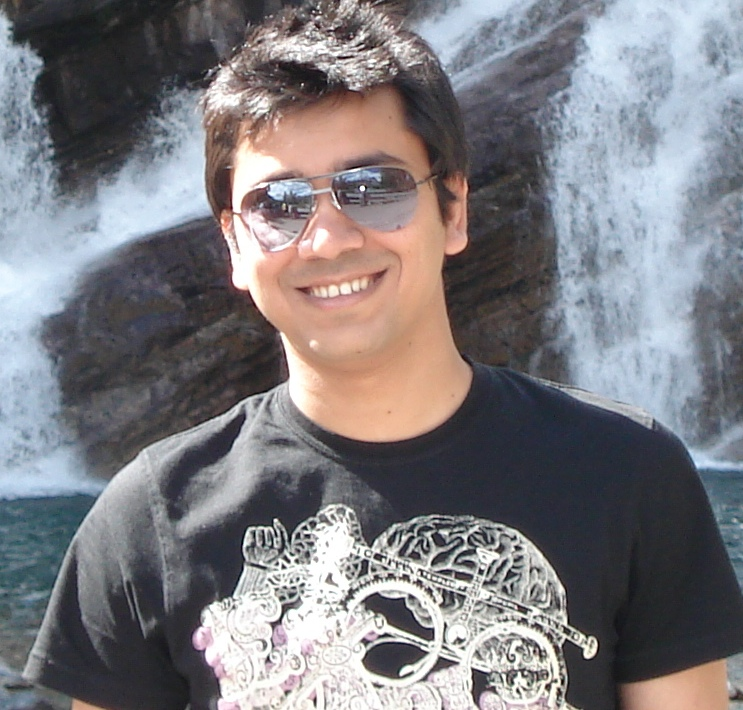
\includegraphics[width=0.16\textwidth]{Picture-019}
%\end{wrapfigure}

\MyName{Shafiq R. Joty}
\MySlogan{Curriculum Vit\ae\ (\today)}

\sepspace

%%% Personal details
%%% ------------------------------------------------------------
\NewPart{}{}

\PersonalEntry{Address}{{Block N4, 2c-111}} 
\hspace{3.04cm} \href{http://scse.ntu.edu.sg/Pages/Home.aspx} {School of Computer Science and Engineering (SCSE)}

\hspace{3.04cm} \href{http://www.ntu.edu.sg} {Nanyang Technological University (NTU)}

\hspace{3.04cm} Singapore

\PersonalEntry{Phone}{(+65) 69041107, 85752318}
\PersonalEntry{Mail}{\href{mailto:srjoty@ntu.edu.sg}{srjoty@ntu.edu.sg}, \href{mailto:rjoty@cs.ubc.ca}{rjoty@cs.ubc.ca}}
\PersonalEntry{WWW}{\href{https://raihanjoty.github.io/}{https://raihanjoty.github.io/}}
\PersonalEntry{Nationality}{\textbf{Canadian}}
\PersonalEntry{h-index}{\textbf{17} (Google Scholar)}
\PersonalEntry{i10-index}{\textbf{26} (Google Scholar)}

\sepspace

\NewPart{Research Interests}{}
\begin{itemize}
 \item Natural Language Processing
   \begin{itemize}

	\item Discourse Analysis 
		\begin{itemize}
 		\item Discourse parsing, Coherence models, Topic models, Conversation models 
    	\end{itemize}
	\item NLP Applications 

      \begin{itemize}
      \item Question answering, Machine translation, Summarization, Sentiment analysis      
      \end{itemize}

   \end{itemize}
 	
 \item Data Science \& Machine Learning

	\begin{itemize}
 	\item Deep learning, Probabilistic graphical models, Representation learning
 	\item Medical informatics, Social computing
    \end{itemize}

% \item Data Mining
%	\begin{itemize}
% 	\item Medical informatics
%    \item Social computing
%    \end{itemize}

\end{itemize}

\NewPart{PROFESSIONAL EMPLOYMENTS}{}

\EducationEntry{\href{https://raihanjoty.github.io/}{Assistant Professor}}{2017-present}{\href{http://www.ntu.edu.sg/Pages/home.aspx} {Nanyang Technological University (NTU)}, Singapore}{}

\EducationEntry{Research Scientist}{2014-2017}{Qatar Computing Research Institute, Doha, Qatar}{}
%{\begin{itemize}\item{Research on discourse parsing, question answering, \newline text summarization and machine translation}\end{itemize}}
%\sepspace
%\EducationEntry{Visiting Scholar}{2014-2015}{Chinese University of Hong Kong, Hong Kong}{}
%{\begin{itemize}\item{Research on deep learning for sentiment analysis}\end{itemize}}
%\sepspace
\EducationEntry{Research \& Teaching Assistant}{2006-2013}{University of British Columbia \\ University of Lethbridge}{}
\EducationEntry{Research Intern}{2010}{Microsoft Research}{}
%\EducationEntry{Research \& Teaching Assistant}{2006–2008}{University of Lethbridge}{}
\EducationEntry{Lecturer}{2005-2006}{Islamic University of Technology, Dhaka, Bangladesh}{}%{\begin{itemize}\item{Taught undergraduate-level courses}\end{itemize}}
%\EducationEntry{Software Developer (Part time)}{2002 - 2005}{Anam Technologies Inc, Dhaka, Bangladesh}{}%{\begin{itemize}\item{Taught undergraduate-level \ExpEntry {,} {} {}


%%% Education
%%% ------------------------------------------------------------
\NewPart{Education}{}

\EducationEntry{Ph.D. (Computer science)}{2008-2013}{University of British Columbia (UBC), Vancouver, Canada}{\href{https://open.library.ubc.ca/cIRcle/collections/ubctheses/24/items/1.0165726}{``Discourse analysis of asynchronous conversations''}\\
{Thesis advisors: \href{https://www.cs.ubc.ca/~carenini/}{Giuseppe Carenini} \& \href{https://www.cs.ubc.ca/~rng/}{Raymond T. Ng}}\\
{Internal committee members: \href{https://www.cs.ox.ac.uk/people/nando.defreitas/} {Nando de Freitas} (now at Oxford) \& \href{http://www.cs.ubc.ca/~rap/} {Rachel Pottinger}}\\ 
{External committee members: \href{http://www.cs.cmu.edu/~cprose/}{Carolyn P. Rosé} (CMU) \& \href {http://amandastent.com/}{Amanda Stent} (Yahoo! Research)}
}
\sepspace
\EducationEntry{M.Sc. (Computer science)}{2006-2008}{University of Lethbridge (UofL), Alberta, Canada}
{\href{https://www.uleth.ca/dspace/handle/10133/666}
{``Answer Extraction for Simple and Complex Questions''}\\
  {Thesis advisor: \href{http://www.cs.uleth.ca/~chali/}{Yllias Chali}}\\
{Other committee members: Sajjad Zahir, Howard Cheng \& Giuseppe Carenini (external)}
}
\sepspace
\EducationEntry{B.Sc. (Computer science)}{2001-2005}{Islamic University of Technology (IUT), Dhaka, Bangladesh}
{CGPA: 4.97/5.00}
\sepspace


\NewPart{Major Honors and Awards}{}

\begin{itemize}

\item \href{http://www.nserc-crsng.gc.ca/Students-Etudiants/PG-CS/BellandPostgrad-BelletSuperieures_eng.asp}{NSERC Alexander Graham Bell Canada Graduate Scholarship\footnote{This award is given only to the top-ranked PhD students across Canada.} (CGS-D)}\\ {$2010-2012$}\hspace{3cm}{$\$35,000$ CAD/Year}
\item \href{https://www.grad.ubc.ca/awards/four-year-doctoral-fellowship-4yf}{Four Year Fellowship (UBC)}\\ {$2010-2013$}\hspace{3cm}{$\$18,000$ CAD/Year}
\item \href{https://www.grad.ubc.ca/awards/affiliated-fellowships}{Faculty of Science Graduate Studies Award (UBC)}\\ {$2010-2013$}\hspace{3cm}{$\$7,200$ CAD/Year}
\item {Microsoft Research Excellent Intern, 2010}
\item {David R. Cheriton Scholarship, University of Waterloo, 2008 [Declined]} 
\item {FS Chia Ph.D. Scholarship, University of Alberta, 2008 [Declined]}
\item {First class 2nd position in BSc}
\item {5th in higher secondary (HSC) \& 11th in secondary (SSC) merit lists}

\end{itemize}



\NewPart{TEACHING EXPERIENCE}{}

\EducationEntry{{Instructor, Nanyang Technological University}} {2017-2018}{\begin{itemize}\item \small Courses Taught: Data Structures (Ugrad), Natural Language Processing (Grad).\end{itemize}}{}

\EducationEntry{{Machine Learning Tutorial  at QCRI} (\href{https://drive.google.com/drive/folders/0B9R_x56MrOrsT3ZwRjFHRHNfaEk}{link} to the lectures)}{2015-2016}{\begin{itemize}\item \small Gave 12 lectures to the scientists at QCRI on ML models: simple discriminative/generative \\ models, latent variable models, directed/undirected graphical models, deep neural networks.\end{itemize}}{}

\EducationEntry{{Teaching Assistant, University of British Columbia}}{2008-2013}{\begin{itemize}\item \small {Courses TAed: Grad NLP, Grad/Ugrad AI, Object Oriented Programming, Intro. to Comp.}\end{itemize}}{}

\EducationEntry{{Teaching Assistant, University of Lethbridge}}{2006-2008}{\begin{itemize}\item \small {Courses TAed: Introduction to Computers.}\end{itemize}}{}

\EducationEntry{{Lecturer, Islamic University of Technology}}{2005-2006}{\begin{itemize}\item \small {Courses Taught: Theory of computation, UNIX prog., Systems prog., OOP.}\end{itemize}}{}


\NewPart{Impact and Visibility}{}

\begin{itemize}

\item \href{http://alt.qcri.org/tools/discourse-parser/}{Discourse Parser for English}\\ {-- \href{http://alt.qcri.org/demos/Discourse_Parser_Demo/} {Demo} -- \href{http://alt.qcri.org/tools/discourse-parser/}{Source Code} -- \href{http://alt.qcri.org/tools/discourse-eval/} {Evaluation metric}}

\item \href{http://alt.qcri.org/tools/speech-act/}{Neural Local Coherence Model}\\ {-- \href{https://github.com/datienguyen/cnn_coherence/}{Source Code}}

\item \href{http://alt.qcri.org/tools/speech-act/}{Discourse-informed Sen2Vec}\\ {-- \href{https://gitlab.com/tksaha/sen2vec}{Source Code \& Data}}


\item \href{http://alt.qcri.org/tools/speech-act/}{Speech act recognizer for synchronous and asynchronous conversations}\\ {-- \href{http://alt.qcri.org/tools/speech-act/}{Source Code} -- \href{http://alt.qcri.org/tools/speech-act/} {Dataset}}

\item \href{http://www.qatarliving.com/betasearch}{Community Question Answering System [Joint work with MIT]}\\ {-- \href{http://www.qatarliving.com/betasearch} {Deployed system} -- \href{http://www.qatarliving.com/betasearch} {Demo} -- \href{http://www.qna.org.qa/en-us/News/16032718350063/QCRI-Collaborates-with-Qatar-Living-to-Improve-Online-Search} {Media coverage}}

\item \href{https://www.cs.ubc.ca/cs-research/lci/research-groups/natural-language-processing/Software.html}{Topic Segmenter \& Labeler for Asynchronous Conversations}\\ {-- \href{https://www.cs.ubc.ca/cs-research/lci/research-groups/natural-language-processing/Software.html} {Source Code and datasets}}

\item \href{https://github.com/CrisisNLP/deep-learning-for-big-crisis-data}{Deep Learning for Crisis Computing}\\ {-- \href{https://github.com/CrisisNLP/deep-learning-for-big-crisis-data}{Source Code} }

\item \href{https://github.com/ppfliu/opinion-target}{Recurrent Neural Models for Fine-grained Opinion Analysis}\\ {-- \href{https://github.com/ppfliu/opinion-target} {Source Code}}





\item \href{https://github.com/Qatar-Computing-Research-Institute/mosesdecoder}{Neural Domain Adaptation Model for Machine Translation}\\ {-- \href{https://github.com/Qatar-Computing-Research-Institute/mosesdecoder} {Source Code} (inside Moses)}


%\item \href{https://github.com/Qatar-Computing-Research-Institute}{Deep Neural Models for Disaster Response}\\ {-- \href{https://github.com/Qatar-Computing-Research-Institute} {Software} is made publicly available}

\item \href{https://github.com/Qatar-Computing-Research-Institute}{Discourse-based Evaluation Metric for Machine Translation}\\ {-- \href{https://github.com/Qatar-Computing-Research-Institute} {Source Code}}


\item \href{https://www.cs.ubc.ca/cs-research/lci/research-groups/natural-language-processing/bc3.html}{The BC3: British Columbia Conversation Corpora}\\ {-- \href{https://www.cs.ubc.ca/cs-research/lci/research-groups/natural-language-processing/bc3.html} {Datasets and annotation framework}}

\end{itemize}







%%% Papers
%%% ------------------------------------------------------------

\vspace{1cm}
\NewPart{Peer-Reviewed Journal Papers}{}

\begin{enumerate}

\item \PaperEntry{\textbf{Shafiq Joty}, Francisco Guzmán, Lluís Màrquez, and Preslav Nakov.}{Discourse Structure in Machine Translation Evaluation.}{Computational Linguistics.}{x}{forthcoming}{2017}.
{}

\item \PaperEntry{\textbf{Shafiq Joty}, Nadir Durrani, Hassan Sajjad, and Ahmed Abdelali.}{Domain Adaptation Using Neural Network Joint Model.}{Journal of Computer Speech and Language (Special Issue on Deep Learning for Machine Translation).}{csl.2016.12.006}{}{2017}
{http://www.sciencedirect.com/science/article/pii/S0885230816301474}

\item \PaperEntry{Francisco Guzmán, \textbf{Shafiq Joty}, Lluís Màrquez, and Preslav Nakov.}{Machine Translation Evaluation with Neural Networks.}{Journal of Computer Speech and Language (Special Issue on Deep Learning for Machine Translation).}{csl.2016.12.005}{}{2016}
{http://www.sciencedirect.com/science/article/pii/S0885230816301693}

\item \PaperEntry{Aarti Sathyanarayana, \textbf{Shafiq Joty}, Luis Fernandez-Luque, Ferda Ofli, Jaideep Srivastava, Ahmed Elmagarmid, Shahrad~Taheri, and Teresa Arora.}{Sleep Quality Prediction From Wearable Data Using Deep Learning}{JMIR Mhealth Uhealth (JMU)}{(4(4):e125)}{JMIR}{2016}
{http://mhealth.jmir.org/2016/4/e125/}

\item \PaperEntry{\textbf{Shafiq Joty}, Giuseppe Carenini and Raymond Ng}{CODRA: A Novel Discriminative Framework for Rhetorical Analysis.}{Computational Linguistics.}{41:3}{385–435, MIT press}{2015}
{http://www.mitpressjournals.org/doi/abs/10.1162/COLI_a_00226\#.VloBH8YgjBE}

\item \PaperEntry{\textbf{Shafiq Joty}, Giuseppe Carenini and Raymond Ng}{Topic Segmentation and Labeling in Asynchronous Conversations.}{Journal of AI Research.}{47}{521-573}{2013}
{https://www.jair.org/media/3940/live-3940-7166-jair.pdf}

\item \PaperEntry{Yllias Chali, Sadid Hasan and \textbf{Shafiq Joty}}{Improving graph-based random walks for complex question answering using syntactic, shallow semantic and extended string subsequence kernels.}{Information Processing and Management.}{47:6}{843–855, Elsevier}{2011} 
{http://www.sciencedirect.com/science/article/pii/S0306457310000877}

\item \PaperEntry{Yllias Chali, \textbf{Shafiq Joty} and Sadid Hasan}{Complex Question Answering: Unsupervised Learning Approaches and Experiments.}{Journal of AI Research.}{35}{1-47}{2009} 
{https://www.jair.org/media/2784/live-2784-4446-jair.pdf} (I was a co-lead author of this paper.)


\end{enumerate}

%\NewPart{Journal Papers Conditionally Accepted}{}

%\begin{enumerate}



%\item \PaperEntry{\textbf{Shafiq Joty}, Lluis Marquez, and Preslav Nakov.}{Joint Multitask Learning for Community Question Answering Using Task-Specific Embeddings.}{Transactions of the Association for Computational Linguistics.}{}{x}{2017}
%{}

%\item \PaperEntry{Tanay Saha, \textbf{Shafiq Joty}, and Mohammad Hasan.}{CON-S2V: A Generic Framework
%for Incorporating Extra-Sentential Context into Sen2Vec.}{Transactions of the Association for Computational Linguistics.}{}{x}{2017}
%{}

%\end{enumerate}

%\NewPart{Journal Papers Under Review}{}

%\begin{enumerate}


%\end{enumerate}

%\newpage
\NewPart{Peer-Reviewed Conference Papers}{[BY YEAR]}

\Large \textbf{2017} \normalsize

\begin{enumerate}

\item \PaperEntry{Tanay Kumar Saha, \textbf{Shafiq Joty} and Mohammad Al Hasan.} {CON-S2V: A Generic Framework for Incorporating Extra-Sentential Context into Sen2Vec.}{In Proceedings of the European Conference on Machine Learning and practice of knowledge discovery in databases} {(ECML-PKDD-2017)}{to appear, Macedonia, Skopje}{2017}  
{https://raihanjoty.github.io/papers/saha-joty-hasan-ecml-17.pdf}

\item \PaperEntry{Tanay Kumar Saha, \textbf{Shafiq Joty}, Naeemul Hassan, and Mohammad Al Hasan.} {Regularized and Retrofitted models for Learning Sentence Representation with Context.}{In Proceedings of the 26th ACM International Conference on Information and Knowledge Management} {(CIKM-2017)}{to appear, Singapore}{2017}  
{http://alt.qcri.org/~sjoty/paper/sen2vec-reg.pdf}

\item \PaperEntry{Dat Tien Nguyen and \textbf{Shafiq Joty} (co-lead author)}{A Neural Local Coherence Model.}{In Proceedings of the 55th Annual Meeting of the Association for Computational Linguistics} {(ACL-2017)}{pages 1320-1330, Vancouver, Canada}{2017}  
{http://www.aclweb.org/anthology/P/P17/P17-1121.pdf}

\item \PaperEntry{\textbf{Shafiq Joty}, Preslav Nakov and Lluís Màrquez}{Cross-language Learning with Adversarial Neural Networks.}{In Proceedings of The SIGNLL Conference on Computational Natural Language Learning} {(CoNLL-2017)}{pages 226-237, Vancouver, Canada}{2017}  
{http://www.aclweb.org/anthology/K/K17/K17-1024.pdf}

\item \PaperEntry{Enamul Hoque, \textbf{Shafiq Joty}, Lluís Màrquez, and Giuseppe Carenini.}{CQAVis: Visual Text Analytics for Community Question Answering.}{In Proceedings of the 22nd annual meeting of the intelligent user interfaces} {(IUI-2017)}{pages 161-172, Limassol, Cyprus}{2017}
{http://dl.acm.org/authorize.cfm?key=N22238}

\item \PaperEntry{Giovanni Da San Martino, Salvatore Romeo, Alberto Barron-Cedeno, Shafiq Joty, Lluís Màrquez, Alessandro Moschitti and Preslav Nakov.}{Cross-Language Question Re-ranking.}{In Proceedings of the 40th International ACM SIGIR Conference on Research and Development in Information Retrieval} {(SIGIR-2017)}{pages 1145-1148, Tokyo, Japan}{2017}
{http://dl.acm.org/citation.cfm?doid=3077136.3080743}

\item \PaperEntry{Dat Tien Nguyen, Kamla Al-Mannai, \textbf{Shafiq Joty}, Hassan Sajjad, Muhammad Imran and Prasenjit Mitra.}{Robust Classification of Crisis-Related Data on Social Networks using Convolutional Neural Networks.}{In Proceedings of the 11-th International AAAI Conference on Weblogs and Social Media } {(ICWSM-2017)}{pages 632-635, Montreal, Canada}{2017}
{http://mimran.me/papers/robust_classification_of_crisis_data_on_social_media_using_cnn_icwsm2017.pdf}

\end{enumerate}

\Large \textbf{2016} \normalsize

\begin{enumerate}


\item \PaperEntry{\textbf{Shafiq Joty} and Enamul Hoque.}{Speech Act Modeling of Written Asynchronous Conversations with Task-Specific Embeddings and Conditional Structured Models.}{In Proceedings of the 54th Annual Meeting of the Association for Computational Linguistics} {(ACL-2016)}{pages 1746-1756, Berlin, Germany}{2016}
{https://www.aclweb.org/anthology/P/P16/P16-1165.pdf}

\item \PaperEntry{\textbf{Shafiq Joty}, Lluís Màrquez and Preslav Nakov.}{Joint Learning with Global Inference for Comment Classification in Community Question Answering.}{In Proceedings of the North American Chapter of the Association for Computational Linguistics: Human Language Technologies} {(NAACL-2016)}{pages 703-713, San Diego, USA}{2016}
{http://m-mitchell.com/NAACL-2016/NAACL-HLT2016/pdf/N16-1084.pdf}

\item \PaperEntry{Nadir Durrani, Hassan Sajjad, \textbf{Shafiq Joty}, and Ahmed Abdelali.}{A Deep Fusion Model for Domain Adaptation in Phrase-based MT.}{In Proceedings of the 26th International Conference on Computational Linguistics} {(COLING-2016)}{to appear, Osaka, Japan}{2016}
{http://coling2016.anlp.jp/}

\item \PaperEntry{Enamul Hoque, \textbf{Shafiq Joty}, Lluís Màrquez, Alberto Barrón-Cedeño, Alessandro Moschitti, Giovanni Da San Martino, Preslav Nakov, Salvatore Romeo and Giuseppe Carenini.}{An Interactive System for Exploring Community Question Answering Forums.}{In Proceedings of the 26th International Conference on Computational Linguistics} {(COLING-2016)}{to appear, Osaka, Japan}{2016}
{http://coling2016.anlp.jp/}

%\item \PaperEntry{\textbf{Shafiq Joty}, Alberto Barrón-Cedeño, Giovanni Da San Martino, Alessandro Moschitti, Lluís Màrquez and Preslav Nakov.}{Global Thread-level Inference for Comment Classification in Community Question Answering.}{In Proceedings of the Conference on Empirical Methods in Natural Language Processing} {(EMNLP-2015)}{pages 573-578, Lisbon, Portugal}{2015}
%{http://aclweb.org/anthology/D/D15/D15-1068.pdf}
\end{enumerate}

\Large \textbf{2015} \normalsize

\begin{enumerate}
\item \PaperEntry{\textbf{Shafiq Joty}, Hassan Sajjad, Nadir Durrani, Kamla Al-Mannai, Ahmed Abdelali and Stephan Vogel.}{How to Avoid Unwanted Pregnancies: Domain Adaptation using Neural Network Models.}{In Proceedings of the Conference on Empirical Methods in Natural Language Processing} {(EMNLP-2015)}{pages 1259-1270, Lisbon, Portugal}{2015}
{http://aclweb.org/anthology/D/D15/D15-1147.pdf}

\item \PaperEntry{\textbf{Shafiq Joty}, Alberto Barrón-Cedeño, Giovanni Da San Martino, Alessandro Moschitti, Lluís Màrquez and Preslav Nakov.}{Global Thread-level Inference for Comment Classification in Community Question Answering.}{In Proceedings of the Conference on Empirical Methods in Natural Language Processing} {(EMNLP-2015)}{pages 573-578, Lisbon, Portugal}{2015}
{http://aclweb.org/anthology/D/D15/D15-1068.pdf}

\item \PaperEntry{Pengfei Liu, \textbf{Shafiq Joty}, and Helen Meng.}{Fine-grained Opinion Mining with Recurrent Neural Networks and Word Embeddings.}{In Proceedings of the Conference on Empirical Methods in Natural Language Processing} {(EMNLP-2015)}{pages 1433-1443, Lisbon, Portugal}{2015}
{http://aclweb.org/anthology/D/D15/D15-1168.pdf}

\item \PaperEntry{Francisco Guzmán, \textbf{Shafiq Joty}, Lluís Màrquez, and Preslav Nakov.}{Pairwise Neural Machine Translation Evaluation.}{In Proceedings of the 53rd annual meeting of the Association for Computational Linguistics} {(ACL-2015)}{pages 805 -814, Beijing, China}{2015}
{https://aclweb.org/anthology/P/P15/P15-1078.pdf}

\item \PaperEntry{Alberto Barrón-Cedeño, Simone Filice, Giovanni Da San Martino, \textbf{Shafiq Joty}, Lluis Marquez, Preslav Nakov and Alessandro Moschitti.}{Thread-level Information for Comment Classification in Community Question Answering.}{In Proceedings of the 53rd annual meeting of the Association for Computational Linguistics} {(ACL-2015)}{pages 687-693, Beijing, China}{2015}
{http://www.aclweb.org/anthology/P15-2113}

\item \PaperEntry{Nadir Durrani, Hassan Sajjad, \textbf{Shafiq Joty}, Ahmed Abdelali and Stephan Vogel.}{Using Joint Models for Domain Adaptation in Statistical Machine Translation.}{In Proceedings of the Association for Machine Translation in the Americas} {(AMTA-2015)}{Miami, USA}{2015}
{http://www.researchgate.net/publication/281556042_Using_Joint_Models_for_Domain_Adaptation_in_Statistical_Machine_Translation}
\end{enumerate}

\Large \textbf{2014} \normalsize

\begin{enumerate}
\item \PaperEntry{\textbf{Shafiq Joty}, Alessandro Moschitti.}{Discriminative Reranking of Discourse Parses Using Tree Kernels.}{In Proceedings of the Conference on Empirical Methods in Natural Language Processing} {(EMNLP-2014)}{pages 2049-2060, Doha, Qatar}{2014}
{http://emnlp2014.org/papers/pdf/EMNLP2014219.pdf}

\item \PaperEntry{Francisco Guzmán, \textbf{Shafiq Joty}, Lluís Màrquez, Alessandro Moschitti, Preslav Nakov and Massimo Nicosia.}{Learning to Differentiate Better from Worse Translations.}{In Proceedings of the Conference on Empirical Methods in Natural Language Processing} {(EMNLP-2014)}{pages 214-220, Doha, Qatar}{2014}
{http://aclweb.org/anthology/D/D14/D14-1027.pdf}

\item \PaperEntry{Iman Saleh, Alessandro Moschitti, Preslav Nakov, Lluís Màrquez and \textbf{Shafiq Joty}.}{Semantic Kernels for Semantic Parsing.}{In Proceedings of the Conference on Empirical Methods in Natural Language Processing} {(EMNLP-2014)}{pages 436-442, Doha, Qatar}{2014}
{http://qcri.org.qa/app/media/4849}

\item \PaperEntry{Francisco Guzmán, \textbf{Shafiq Joty}, Lluís Màrquez, and Preslav Nakov.}{Using Discourse Structure Improves Machine Translation Evaluation.}{In Proceedings of the 52nd annual meeting of the Association for Computational Linguistics} {(ACL-2014)}{pages 687-698, Baltimore, USA}{2014}
{http://qcri.org.qa/app/media/4865}

\item \PaperEntry{Iman Saleh, \textbf{Shafiq Joty}, Lluís Màrquez, Alessandro Moschitti, Preslav Nakov, Scott Cyphers and Jim Glass.}{A Study of Using Syntactic and Semantic Structures for Concept Segmentation and Labeling.}{In Proceedings of the 25th International Conference on Computational Linguistics} {(COLING-2014)}{pages 193-202, Dublin, Ireland}{2014}
{http://anthology.aclweb.org/C/C14/C14-1020.pdf}
\end{enumerate}


\Large \textbf{2013} \normalsize

\begin{enumerate}

\item \PaperEntry{\textbf{Shafiq Joty}, Giuseppe Carenini, Raymond Ng and Yashar Mehdad.}{Combining Intra- and Multi-sentential Rhetorical Parsing for Document-level Discourse Analysis.}{In Proceedings of the 51st Annual Meeting of the Association for Computational Linguistics.} {(ACL-2013)}{pages 486-496, Sofia, Bulgaria}{2013}
{http://www.aclweb.org/anthology/P13-1048}

\item \PaperEntry{Yashar Mehdad, Giuseppe Carenini, Raymond Ng and \textbf{Shafiq Joty}.}{Towards Topic Labeling with Phrase Entailment and Aggregation.}{In Proceedings of the North American Chapter of the Association for Computational Linguistics: Human Language Technologies.} {(NAACL-2013)}{pages 179-189, Atlanta, USA}{2013}
{http://www.aclweb.org/anthology/N13-1018}

\item \PaperEntry{Maryam Tavafi, Yashar Mehdad, \textbf{Shafiq Joty}, Giuseppe Carenini, Raymond Ng.}{Dialogue Act Recognition in Synchronous and Asynchronous Conversations.}{In Proceedings of the 14th Annual Meeting of the Special Interest Group on Discourse and Dialogue.} {(SIGDIAL-2013)}{pages 117-121, Metz, France.}{2013}
{http://www.aclweb.org/anthology/W13-4017}

\end{enumerate}

\Large \textbf{2012} \normalsize
\begin{enumerate}
\item \PaperEntry{\textbf{Shafiq Joty}, Giuseppe Carenini and Raymond Ng.}{A Novel Discriminative Framework for Sentence-Level Discourse Analysis.}{In Proceedings of the Conference on Empirical Methods in Natural Language Processing and the Conference on Natural Language Learning.} {(EMNLP-2012)}{pages 904-915, Jeju, Korea}{2012}
{https://aclweb.org/anthology/D/D12/D12-1083.pdf}
\end{enumerate}

\Large \textbf{2011} \normalsize
\begin{enumerate}

\item \PaperEntry{\textbf{Shafiq Joty}, Giuseppe Carenini and Chin-Yew Lin.}{Unsupervised Modeling of Dialog Acts in Asynchronous Conversations.}{In Proceedings of the twenty second International Joint Conference on Artificial Intelligence.} {(IJCAI-2011)}{pages 1807-1813, Barcelona, Spain}{2011}
{http://dl.acm.org/citation.cfm?id=2283705}

\item \PaperEntry{\textbf{Shafiq Joty}, Giuseppe Carenini, Gabriel Murray and Raymond Ng.}{Supervised Topic Segmentation of Email Conversations.}{In Fifth International AAAI Conference on Weblogs and Social Media.} {(ICWSM-2011)}{pages 530-533, Barcelona, Spain}{2011}
{https://www.aaai.org/ocs/index.php/ICWSM/ICWSM11/paper/viewFile/2882/3228}

\item \PaperEntry{Nicholas FitzGerald, Giuseppe Carenini, Gabriel Murray and \textbf{Shafiq Joty}.}{Exploiting Conversational Features to Detect High-Quality Blog Comments.}{In Proceedings of the Canadian Conference on Artificial Intelligence} {(CAI-2011)}{pages 122-127, St. Johns, Newfoundland}{2011}
{http://link.springer.com/chapter/10.1007/978-3-642-21043-3_15}
\end{enumerate}

\Large \textbf{2010} \normalsize
\begin{enumerate}
\item \PaperEntry{\textbf{Shafiq Joty}, Giuseppe Carenini, Gabriel Murray and Raymond Ng.}{Exploiting Conversation Structure in Unsupervised Topic Segmentation for Emails.}{In Proceedings of the Conference on Empirical Methods in Natural Language Processing and the Conference on Natural Language Learning.} {(EMNLP-2010)}{pages 388-398, Massachusetts, USA.}{2010}
{https://www.aclweb.org/anthology/D/D10/D10-1038.pdf}
\end{enumerate}

\Large \textbf{2009} \normalsize
\begin{enumerate}

\item \PaperEntry{Yllias Chali, Sadid Hasan and \textbf{Shafiq Joty}.}{Do Automatic Annotation Techniques Have Any Impact on Supervised Complex Question Answering?}{In Proceedings of the ACL-IJCNLP 2009 Conference.} {(ACL-2009)}{pages 329-332, Suntec, Singapore.}{2009}
{http://www.aclweb.org/anthology/P09-2083}

\item \PaperEntry{Yllias Chali, Sadid Hasan and \textbf{Shafiq Joty}.}{A SVM-Based Ensemble Approach to Multi-Document Summarization.}{In Proceedings of the 22nd Canadian Conference on Artificial Intelligence } {(CAI-2009)}{pages 329-332, Kelowna,Canada.}{2009}
{http://link.springer.com/chapter/10.1007\%2F978-3-642-01818-3_23}

\item \PaperEntry{Yllias Chali, Sadid Hasan and \textbf{Shafiq Joty}.}{Supervised Approaches to Complex Question Answering.}{In Proceedings of Conference of the Pacific Association for Computational Linguistics} {(PACLING-2009)}{pages 121-126, Sapporo, Japan.}{2009}
{http://www.sadidhasan.com/sadid-PACLING.pdf}

\end{enumerate}

\Large \textbf{2008} \normalsize
\begin{enumerate}

\item \PaperEntry{Yllias Chali and \textbf{Shafiq Joty}.}{Selecting Sentences for Answering Complex Questions.}{In Proceedings of the Conference on Empirical Methods in Natural Language Processing} {(EMNLP-2008)}{pages 304-313, Hawaii, USA.}{2008}
{http://www.aclweb.org/anthology/D08-1032}
(I was a co-lead author.)

\item \PaperEntry{Yllias Chali and \textbf{Shafiq Joty}.}{Improving the Performance of the Random Walk Model for Answering Complex Questions.}{In Proceedings of the 46th Annual Meeting of the Association for Computational Linguistics: Human Language Technologies} {(ACL-2008)}{pages 9-12, OH, USA.}{2008}
{http://dl.acm.org/citation.cfm?id=1557694}
(I was a co-lead author.)

\item \PaperEntry{Yllias Chali and \textbf{Shafiq Joty}.}{Exploiting Syntactic and Shallow Semantic Kernels to Improve Random Walks for Complex Question Answering.}{In Proceedings of the 20th IEEE Int'l Conference on Tools with Artificial Intelligence} {(ICTAI-2008)}{pages 123-130, OH, USA.}{2008}
{https://www.computer.org/csdl/proceedings/ictai/2008/3440/02/3440b123.pdf}
(I was a co-lead author.)

\item \PaperEntry{Yllias Chali and \textbf{Shafiq Joty}.}{Answering Complex Questions Using Query-focused Summarization Technique.}{In Proceedings of the 20th IEEE Int'l Conference on Tools with Artificial Intelligence} {(ICTAI-2008)}{pages 131-134, OH, USA.}{2008}
{https://www.computer.org/csdl/proceedings/ictai/2008/3440/02/3440b131.pdf}
(I was a co-lead author.)

\item \PaperEntry{Yllias Chali and \textbf{Shafiq Joty}.}{Unsupervised Approach for Selecting Sentences in Query-based Summarization.}{In Proceedings of the 21st FLAIRS conference} {(FLAIRS-2007)}{pages 47-52, Florida, USA.}{2008}
{http://www.aaai.org/Library/FLAIRS/2008/flairs08-019.php}
(I was a co-lead author.)

\item \PaperEntry{Gabriel Murray, \textbf{Shafiq Joty}, Giuseppe Carenini and Raymond Ng.}{The University of British Columbia at TAC 2008.}{n Proceedings of the Text Analysis Conference} {(TAC-2008)}{Rochester, USA.}{2008}
{http://www.nist.gov/tac/publications/2008/participant.papers/UBC.proceedings.pdf}

\item \PaperEntry{Yllias Chali and \textbf{Shafiq Joty} and Sheikh Sadid-Al-Hasan.}{UofL at TAC 2008 Update Summarization and Question Answering.}{n Proceedings of the Text Analysis Conference} {(TAC-2008)}{Rochester, USA.}{2008}
{http://www.nist.gov/tac/publications/2008/participant.papers/UofL.proceedings.pdf}

\end{enumerate}

\Large \textbf{2007} \normalsize
\begin{enumerate}

\item \PaperEntry{Yllias Chali and \textbf{Shafiq Joty}.}{University of Lethbridge’s Participation in DUC-2007 Main Task.}{In Proceedings of the Document Understanding Conference} {(DUC-2007)}{Rochester, USA.}{2007}
{http://duc.nist.gov/pubs/2007papers/ulethbridge.pdf}
(I was a co-lead author.)

\item \PaperEntry{Yllias Chali and \textbf{Shafiq Joty}.}{University of Lethbridge’s Participation in TREC-2007 Main Task.}{In Proceedings of the Sixteenth Text REtrieval Conference} {(TREC-2007)}{Gaithersburg, USA.}{2007}
{http://trec.nist.gov/pubs/trec16/papers/ulethbridge.qa.final.pdf}
(I was a co-lead author.)

\item \PaperEntry{\textbf{Shafiq Joty} and Sadid Hasan.}{Advances in Focused Retrieval: A General Review.} {In Proceedings of the 10th IEEE International Conference on Computer and Information Technology}{(ICCIT-2007)}{pages 1-5, Dhaka, Bangladesh.}{2007}
{http://ieeexplore.ieee.org/xpls/abs_all.jsp?arnumber=4579357&tag=1}

\end{enumerate}

\Large \textbf{2005} \normalsize
\begin{enumerate}

\item \PaperEntry{\textbf{Shafiq Joty}, Abdullah Al Hasib and Kaisar Imam.} {A Disruption Tolerant Content-Aware Video Streaming Approach for Real-Time Multimedia Data with Appropriate Error Concealment Method.}{In proceedings of the 8th International Conference on Computer and Information Technology}{(ICCIT-2005)}{Dhaka, Bangladesh.}{2005}
{http://ieeexplore.ieee.org/xpls/abs_all.jsp?arnumber=4579357&tag=1}

\end{enumerate}

%\NewPart{Conference Papers Under Review}{}

%\begin{enumerate}

%\item \PaperEntry{Dat Tien Nguyen, Kamela Ali Al Mannai, \textbf{Shafiq Joty}, Hassan Sajjad, Muhammad Imran, and Prasenjit Mitra.}{Rapid Classification of Crisis-Related Data on Social Networks using Convolutional Neural Networks.} {In IEEE Big Data.} {x}{x}{2016}
%{}

%\item \PaperEntry{Tanay Kumar Saha, \textbf{Shafiq Joty}, and Naeemul Hassan.}{Discourse Informed Sen2Vec.} {Anonymous.} {x}{x}{2016}
%{}

%\end{enumerate}


\NewPart{Peer-Reviewed Workshop Papers}{}


\begin{enumerate}

\item \PaperEntry{Dat Nguyen, \textbf{Shafiq Joty}, Basma Boussaha, and Maarten de Rijke.}{Thread Reconstruction in Conversational Data using Neural Coherence Models.} {In Proceedings of the Neu-IR 2017 SIGIR Workshop on Neural Information Retrieval} {(NeuIR'17)} {Tokyo, Japan}{2017}
{https://raihanjoty.github.io/papers/nguyen-joty-boussaha-rijke-neuir-17.pdf}

\item \PaperEntry{Alberto Barrón-Cedeño, Giovanni Da San Martino, \textbf{Shafiq Joty}, Alessandro Moschitti, Fahad Al-Obaidli, Salvatore Romeo, Kateryna Tymoshenko and Antonio Uva.}{ConvKN at SemEval-2016 Task 3: Answer and Question Selection for Question Answering on Arabic and English Fora.} {In Proceedings of the 10th International Workshop on Semantic Evaluation.} {(SemEval 2016)} {San Diego, USA}{2016}
{https://aclweb.org/anthology/S/S16/S16-1138.pdf}
\textcolor{red}{(2$^{nd}$ place in both English \& Arabic subtasks of Task 3)}

\item \PaperEntry{Giovanni Da San Martino, Alberto Barrón-Cedeño, Salvatore Romeo, Alessandro Moschitti, \textbf{Shafiq Joty},  Fahad Al-Obaidli,  Kateryna Tymoshenko and Antonio Uva.}{Addressing Community Question Answering in English and Arabic.} {In Second WebQA workshop.} {(SIGIR-WebQA 2016)} {Pisa, Italy}{2016}
{http://plg2.cs.uwaterloo.ca/~avtyurin/WebQA2016/papers/invitedPaper2.pdf}

\item \PaperEntry{Dat Tien Nguyen, \textbf{Shafiq Joty}, Muhammad Imran, Hassan Sajjad, and Prasenjit Mitra.}{Applications of Online Deep Learning for Crisis Response Using Social Media Information.} {In the 4th International Workshop on Social Web for Disaster Management (co-located with CIKM 2016),} {(SWDM 2016)} {Indianapolis, USA}{2016}
{https://arxiv.org/abs/1610.01030}

\item \PaperEntry{Massimo Nicosia, Simone Filice, Alberto Barrón-Cedeño, Iman Saleh, Hamdy Mubarak, Wei Gao, Preslav Nakov, Giovanni Da San Martino, Alessandro Moschitti, Kareem Darwish, Lluís Màrquez, \textbf{Shafiq Joty} and Walid Magdy.}{QCRI: Answer Selection for Community Question Answering - Experiments for Arabic and English.} {In Proceedings of the 9th International Workshop on Semantic Evaluation.}{(SemEval-2015)}{pages 203-209, Denver, USA}{2015}
{http://qcri.org.qa/app/media/4829}
\textcolor{red}{(Winner in Arabic and 3$^{rd}$ place in English subtask of Task 3)}

\item \PaperEntry{\textbf{Shafiq Joty}, Francisco Guzman, Lluis Marquez and Preslav Nakov.}{DiscoTK: Using Discourse Structure for Machine Translation Evaluation.}{In Proceedings of the Ninth Workshop on Statistical Machine Translation} {(WMT-2014)}{pages 402-408, Baltimore, USA}{2014}
{https://www.aclweb.org/anthology/W/W14/W14-3352.pdf}
\textcolor{red}{(Winner of the metric task.)}

\item \PaperEntry{Enamul Hoque, Giuseppe Carenini and \textbf{Shafiq Joty}.}{Interactive Exploration of Asynchronous Conversations: Applying a User-centered Approach to Design a Visual Text Analytic System.} {In Proceedings of the Workshop on Interactive Language Learning, Visualization, and Interfaces}{(ILLVI-2014)}{pages 45-52, Baltimore, USA.}{2014}
{http://nlp.stanford.edu/events/illvi2014/papers/hoque-illvi2014.pdf}

\item \PaperEntry{\textbf{Shafiq Joty}, Giuseppe Carenini and Raymond Ng.}{Automatic Topic Labeling in Asynchronous Conversations.} {The Pacific Northwest Regional NLP Workshop}{(NWNLP-2012)}{Microsoft Research, Redmond, USA.}{2012}
{http://dada.cs.washington.edu/nw-nlp-2012/papers/NWTopicLabel2012_Final.pdf}

\item \PaperEntry{Wei Jin, \textbf{Shafiq Joty}, Giuseppe Carenini and Raymond Ng.}{Detecting Informative Blog Comments using Tree Structured Conditional Random Fields.} {The Pacific Northwest Regional NLP Workshop}{(NWNLP-2012)}{Microsoft Research, Redmond, USA.}{2012}
{http://dada.cs.washington.edu/nw-nlp-2012/papers/Tree_CRF_CameraReady.pdf}

\item \PaperEntry{\textbf{Shafiq Joty}, Giuseppe Carenini, Gabriel Murray and Raymond Ng.}{Exploiting Conversation Features for Finding Topics in Emails.} {The Pacific Northwest Regional NLP Workshop}{(NWNLP-2010)}{Microsoft Research, Redmond, USA.}{2010}
{http://depts.washington.edu/uwcl/nw-nlp-2010/papers/JotyEtAl_Oral.pdf}

\item \PaperEntry{\textbf{Shafiq Joty}, Giuseppe Carenini, Gabriel Murray and Raymond Ng.}{Finding Topics in Emails: Is LDA enough?} {NIPS-2009 workshop on applications for topic models: text and beyond.}{(NIPS-2009)}{Whistler, Canada}{2009}
{http://depts.washington.edu/uwcl/nw-nlp-2010/papers/JotyEtAl_Oral.pdf}

\item \PaperEntry{Yllias Chali and \textbf{Shafiq Joty}.}{Word Sense Disambiguation Using Lexical Cohesion.} {In Proceedings of the 4th International Conference on Semantic Evaluations}{(SemEval-2007)}{pages 476-479, Prague, Czech Republic.}{2007}
{http://www.aclweb.org/anthology/S07-1106}

\end{enumerate}


\NewPart{Research Grants}{}

\begin{enumerate}
\item \FundingEntry{Multilingual Multimodal Language Processing Using Generative Adversarial Autoencoders.} {Targeted to the Tier-1 program.} {Collaboration with UBC (Canada) and SMU (Singapore)}{Aug, 2017}
{}

\item \FundingEntry{Discourse Analysis and Its Applications in Medical Texts.} {Targeted to the Tier-2 program.} {Collaboration with UBC (Canada) and NUS (Singapore)}{Aug, 2017}
{}

\item \FundingEntry{A Computational Exploration of the Social Dynamics of Small Groups: Hypergraphs, Tensors, and Deep Learning.} {Targeted to the NSF IIS Core program.} {Collaboration with the University of Minnesota}{Oct, 2017}
{}
\end{enumerate}



\NewPart{Invited Talks}{}
\begin{enumerate}

\item\TalkEntry{``Structured Predictions for Discourse Analysis and Applications in Natural Language Processing'', University of Calgary} {Calgary, Canada}{Mar. 2017}{}

\item\TalkEntry{``Structured Predictions for Discourse Analysis and Applications in Natural Language Processing'', University of Waterloo} {Waterloo, Canada}{Feb. 2017}{}

\item\TalkEntry{``Structured Predictions for Discourse Analysis and Applications in Natural Language Processing'', Nanyang Technological University (NTU)} {Singapore}{Nov. 2016}{}

\item\TalkEntry{``Introduction to Machine Learning'', Global Entrepreneurship Week} {Doha}{Nov. 2015}{}
\item\TalkEntry{``Discourse Analysis \& its Applications''} {Chinese University of Hong Kong.}{Oct. 2015}{}
\item\TalkEntry{``CODRA: A Complete Discriminative Framework for Rhetorical Analysis''} {Universite Paul Sabatier, Toulouse, France.}{Sep. 2014}{}

\item\TalkEntry{``Discourse Analysis of Asynchronous Conversations''} {University of British Columbia, Vancouver, Canada.}{Dec. 2013}{}

\item\TalkEntry{``Intra- and Multi-sentential Rhetorical Parsing for Document-level Discourse Analysis''} {NSERC Business Intelligence Network AGM, IBM Software Labs, Canada.}{Nov. 2012}{}

\item\TalkEntry{``A Novel Discriminative Framework for Sentence-Level Discourse Analysis''} {NW-NLP workshop, Microsoft Research Redmond.}{May, 2012}{}

\item\TalkEntry{``Discourse Analysis of Asynchronous Conversations (e.g., emails, blogs)''} {Business Intelligence (BI) Workshop-NSERC BIN Watson, IBM Watson center}{Feb, 2012}{}

\item\TalkEntry{``Discourse Analysis of Asynchronous Conversations (e.g., emails, blogs)''} {UBC Social Network Group}{Feb, 2012}{}

\item\TalkEntry{``Unsupervised Modeling of Dialog Acts in Asynchronous Conversations''} {UBC Laboratory for Computational Intelligence (LCI) Forum Talk}{Apr, 2011}{}

\item\TalkEntry{``Topic and Dialog Act Modeling of Asynchronous Conversations''} {Microsoft Research Asia}{Nov, 2010}{}

\item\TalkEntry{``What are they talking about?" Finding Topics in Email Conversations''} {UBC Laboratory for Computational Intelligence Forum (LCI) Talk}{Feb, 2010}{}

\item\TalkEntry{``Answering Simple and Complex Questions''} {University of Alberta NLP Group}{Jan, 2008}{}

\end{enumerate}

\NewPart{Service}{}

\begin{enumerate}
\item Reviewing: TACL [2015-2017], ACL/EMNLP/SigDial/*SEM/NAACL/IJCAI/IUI/KDD.
\item Associate VP position in the Bangladesh Students’ Association, UBC (2009-2010).
\item Organizing committee member of EMNLP-2014, ICCIT-2005.
%\item Student volunteer of IJCAI-2011, ACL-2009.
\end{enumerate}

\NewPart{Professional Membership}{}

\begin{itemize}
\item ACL, SIGDAT, SIGGEN, SIGSEM, ACM, IEEE.
\end{itemize}

%\NewPart{TECHNICAL SKILLS}{}

%\begin{itemize}
%\item Programming Languages: Theano, Python, Perl, C/C++, Matlab.
%\item Operating System experience: Mac, Linux, Windows.
%\end{itemize}


\NewPart{Students}{}
\begin{enumerate}
\item {} {Tasnim Mohiuddin} (PhD at NTU, Singapore) Aug, 2017 - Present.
\item {} {M Saiful Bari} (PhD at NTU, Singapore) Aug, 2017 - Present.
\item \href{http://www.cs.ubc.ca/~enamul/index.html} {Enamul Hoque} (Postdoc at Stanford, USA) Feb, 2016 - May, 2016. 
\item  {Ankit Sharma} (PhD student at University of Minnesota, USA) July, 2016 - Present. 
\item  {Aarti Sathyanarayana} (PhD student at University of Minnesota, USA) July, 2016 - Present. 
\item  {Karan Agarwal} (PhD student at University of Minnesota, USA) June, 2017 - Present. 
\item  {Dat Tien Nguyen} (PhD student at University of Amsterdam, NL) Oct, 2016 - Present. 
\item  {Basma El Amel Boussaha} (PhD student at University of Nantes, FR) Oct, 2016 - Present. 
\item \href{https://www.linkedin.com/in/tanaykumarsaha} {Tanay Saha} (PhD student at IUPUI, USA) June, 2016 - Present. 
\item \href{https://www.linkedin.com/in/pengfei-liu-35335333} {Pengfei Liu} (PhD student at CUHK, Hong Kong) Feb, 2015 - Present. 
\item  {Sameer Khurana} (PhD student at MIT, USA) Sep, 2016 - Present. 
\item {Kamela Al Mannai} (QSTP leadership program) 2014 - present
\item \href{https://www.linkedin.com/in/maryamtavafi} {Mariyam Tavafi} (MSc 2013 @UBC), now a software engineer at Google. 
\item {David Jin} (MSc 2013 @UBC), now a software engineer at Amazon.
\end{enumerate}

\NewPart{References}{}

\begin{tabular}{lr}
% Referee 1
\\
\begin{minipage}[t]{3.5in}
\href{https://www.cs.ubc.ca/~carenini/} {Dr. Giuseppe Carenini}\\
Associate Professor\\ 
Dept. of Computer Science \\ 
University of British Columbia\\
2366 Main Mall, Vancouver, B.C.\\
Canada V6T 1Z4 \\
\Telefon\ +1 (604) 822-5109\\
\Letter\ \href{mailto:carenini@cs.ubc.ca}{carenini@cs.ubc.ca}
\end{minipage}
&
% Referee 2
\begin{minipage}[t]{3.5in}
\href{https://www.cs.ubc.ca/~rng/} {Dr. Raymond T. Ng}\\
Professor \\ 
Director of Data Science Institute \\
Dept. of Computer Science \\ 
University of British Columbia\\
2366 Main Mall, Vancouver, B.C.\\
Canada V6T 1Z4 \\
\Telefon\ +1 (604) 822-2394\\
\Letter\ \href{mailto:rng@cs.ubc.ca}{rng@cs.ubc.ca}
\end{minipage}
\\
\\
\\
\\
% Referee 3
\begin{minipage}[t]{3.5in}
\href{http://dmr.cs.umn.edu/people2.html} {Dr. Jaideep Srivastava}\\
Research Director at the Social Computing Group \\
Qatar Computing Research Institute, HBKU\\
(Professor, University of Minnesota)\\
Qatar Foundation, Doha, Qatar 5825\\
\Letter\ \href{mailto:jsrivastava@qf.org.qa}{jsrivastava@qf.org.qa}
\end{minipage}
&
\begin{minipage}[t]{3.5in}
\href{http://qcri.org.qa/page?name=Lluis_Marquez&a=117&pid=145&lang=en-CA} {Dr. Lluís Màrquez}\\
Principal Scientist at the ALT Research Group\\
Qatar Computing Research Institute, HBKU\\
(Associate Professor, UPC, Barcelona)\\ 
Qatar Foundation, Doha, Qatar 5825\\
\Telefon\ +974 33225787\\
\Letter\ \href{mailto:lmarquez@qf.org.qa}{lmarquez@qf.org.qa}
\end{minipage}
%\\
%\\
%\\
%\begin{minipage}[t]{3.5in}
%\href{http://www.cs.uleth.ca/~chali} {Dr. Yllias Chali}\\
%Professor\\ 
%Dept. of Computer Science \\ 
%University of Lethbridge\\
%4401 University Dr W, Lethbridge, AB\\
%Canada T1K 6T5\\
%\Telefon\ +1 (403) 329-2331\\
%\Letter\ \href{mailto:yllias.chali@uleth.ca}{yllias.chali@uleth.ca}
%\end{minipage}




\end{tabular}






%\newpage

\end{document}
